See Fig. \ref{fig:3.8.3_rain}.
The velocity of rain and velocity of woman are
\begin{align}
\vec{v_r} &= \myvec{0\\-35}
\\
\vec{v_w} &= \myvec{-12\\0}
\end{align}
The relative velocity of rain w.r.t woman is given as
\begin{align}
\vec{v_{r_w}} &=\vec{v_r}- \vec{v_w}
\\
&=\myvec{12\\-35}
\end{align}
So the woman must hold the umbrella along the direction of $-\vec{v_{r_w}}$
Thus, the desired angle is 
\begin{align}
\theta={\tan}^{-1}\brak{\frac{12}{35}}
\end{align}
The following python code generates Fig. \ref{fig:3.8.3_rain}. 
%
\begin{lstlisting}
solutions/3/codes/line/rain/rain.py
\end{lstlisting}
\begin{figure}[!ht]
\centering
\includegraphics[width=\columnwidth]{./solutions/3/codes/line/rain/pyfigs/rain.eps}
\caption{Direction of umbrella}
\label{fig:3.8.3_rain}
\end{figure}
